\ifx\allfiles\undefined
\documentlecture[12pt, a4paper, oneside, UTF8]{ctexbook}  %  这一句是新增加的
\usepackage[dvipsnames]{xcolor}
\usepackage{amsmath}   % 数学公式
\usepackage{graphicx}
\usetikzlibrary{arrows, calc, decorations.pathmorphing}
\allowdisplaybreaks % 允许公式跨页换行
\newcommand{\pa}{\partial}
\newcommand{\mathminus}{\!\!-\!\!} % 数学环境连字符
\newcommand{\vsup}[1]{\raisebox{-0.1ex}{$\scriptstyle #1$}}
\newcommand{\lsup}[1]{\raisebox{-0.85ex}{$\scriptstyle #1$}}


\begin{document}
%
 % 单独编译时,其实不用编译封面目录之类的,如需要不注释这句即可
\else
\fi
%  ↓↓↓↓↓↓↓↓↓↓↓↓↓↓↓↓↓↓↓↓↓↓↓↓↓↓↓↓ 正文部分
\chapter{chemical potentials and multicomponent equilibria}
\begin{zhu}
    双下角标表示纯物质的性质,单下角标表示混合物中该组分的性质,下角标中用逗号隔开表示对其后的性质求偏导。
\end{zhu}
\section{lecture 11-2}
\begin{thm}
    Summary of SES relations
    \begin{enumerate}
        \item (small systems) (Mixtures)
        \begin{align*}
            Eu &= E - TS + pV - \vec{\mu}\cdot \vec{n} = F + pV - \vec{\mu}\cdot \vec{n} = G - \vec{\mu}\cdot \vec{n} = H - TS - \vec{\mu}\cdot \vec{n} \\
            dEu &= -S dT + V dp - \vec{n}\cdot d\vec{\mu} \Rightarrow Eu = Eu(T, p, \vec{\mu}) \\
            deu &= \frac{1}{n} dEu - Eu \frac{dn}{n^2} = -s dT + v dp - \vec{y} \cdot d\vec{\mu} - eu \frac{dn}{n}\\
             &\Rightarrow eu = eu(T, p, \vec{\mu}, n) = \frac{n_0}{n} eu(T, p, \vec{\mu}, n_0) \\
            de &= \frac{1}{n} dE - E \frac{dn}{n^2} = T ds - p dv + \vec{\mu} \cdot d\vec{y} - eu \frac{dn}{n} \Rightarrow e = e(s, v, \vec{y}, n) \\
            df &= \frac{1}{n} dF - F \frac{dn}{n^2} = -s dT + p dv + \vec{\mu} \cdot d\vec{y} - eu \frac{dn}{n} \Rightarrow f = f(T, v, \vec{y}, n) \\
            dg &= \frac{1}{n} dG - G \frac{dn}{n^2} = -s dT + v dp + \vec{\mu} \cdot d\vec{y} - eu \frac{dn}{n} \Rightarrow g = g(T, p, \vec{y}, n) \\
            dh &= \frac{1}{n} dH - H \frac{dn}{n^2} = T ds + v dp + \vec{\mu} \cdot d\vec{y} - eu \frac{dn}{n} \Rightarrow h = h(s, p, \vec{y}, n)
        \end{align*}
        \item (large n limit) (Mixtures)
        \begin{align*}
            Eu = 0  &\Rightarrow  E - TS + pV - \vec{\mu}\cdot \vec{n} = 0 \quad \boxed{\text{Euler relation}} \\
        &\Rightarrow  \vec{\mu}\cdot \vec{n} = G = H - TS = F + pV = E - TS + pV \\
        dEu &= -S dT + Vdp - \vec{n}\cdot  d\vec{\mu} = 0 \\
        &\Rightarrow  d\mu = -s dT + vdp \quad \boxed{\text{Gibbs-Duhem relation}} \\
        de &= \frac{1}{n} dE - E \frac{dn}{n^2} = T ds - p dv + \vec{\mu} \cdot d\vec{y}  \Rightarrow e = e(s, v, \vec{y}) \\
        df &= \frac{1}{n} dF - F \frac{dn}{n^2} = -s dT + p dv + \vec{\mu} \cdot d\vec{y}  \Rightarrow f = f(T, v, \vec{y}) \\
        dg &= \frac{1}{n} dG - G \frac{dn}{n^2} = -s dT + v dp + \vec{\mu} \cdot d\vec{y}  \Rightarrow g = g(T, p, \vec{y}) \\
        dh &= \frac{1}{n} dH - H \frac{dn}{n^2} = T ds + v dp + \vec{\mu} \cdot d\vec{y}  \Rightarrow h = h(s, p, \vec{y})
        \end{align*}
        \item (small systems) (Pure substances)
        \begin{align*}
            Eu &= E - TS + pV - \mu n = F + pV - \mu n = G - \mu n = H - TS - \mu n \\
dEu &= -S dT + V dp - n d\mu \Rightarrow Eu = Eu(T, p, \mu) \\
deu &= \frac{1}{n} dEu - \frac{dn}{n^2} = -s dT + v dp - d\mu - eu \frac{dn}{n} \\
&\Rightarrow eu = eu(T, p, \mu, n) = \frac{n_0}{n} eu(T, p, \mu, n_0) \\
de &= \frac{1}{n} dE - E \frac{dn}{n^2} = T ds - p dv - eu \frac{dn}{n} \Rightarrow e = e(s, v, n) \\
df &= \frac{1}{n} dF - F \frac{dn}{n^2} = -s dT + p dv - eu \frac{dn}{n} \Rightarrow f = f(T, v, n) \\
dg &= \frac{1}{n} dG - G \frac{dn}{n^2} = -s dT + v dp - eu \frac{dn}{n} \Rightarrow g = g(T, p, n) \\
dh &= \frac{1}{n} dH - H \frac{dn}{n^2} = T ds + v dp - eu \frac{dn}{n} \Rightarrow h = h(s, p, n)
\end{align*}
        \item (large n limit) (Pure substances)
        \begin{align*}
        Eu &= 0  \Rightarrow E - TS + pV - \mu n = 0 \quad \boxed{\text{Euler relation}}\\
        &\Rightarrow \mu n = G = H - TS = F + pV = E - TS + pV \\
dEu &= -S dT + Vdp - n du = 0  \Rightarrow d\mu = -s dT + vdp \quad \boxed{\text{Gibbs-Duhem relation}} \\
        de &= \frac{1}{n} dE - E \frac{dn}{n^2} = T ds - p dv  \Rightarrow e = e(s, v) \\
        df &= \frac{1}{n} dF - F \frac{dn}{n^2} = -s dT + p dv  \Rightarrow f = f(T, v) \\
        dg &= \frac{1}{n} dG - G \frac{dn}{n^2} = -s dT + v dp  \Rightarrow g = g(T, p) \Rightarrow \mu =\mu (T,p) \\
        dh &= \frac{1}{n} dH - H \frac{dn}{n^2} = T ds + v dp  \Rightarrow h = h(s, p)
        \end{align*}
    \end{enumerate}
    \begin{zhu}
    大写字母表示系统中全部的该性质,小写字母表示单位摩尔的该性质。
    \end{zhu}
\end{thm}
\begin{thm}
    \textbf{Partial properties} from the chemical potentials
    \begin{align*}
        dG &= -S \, dT + V \, dp + \mu \cdot dn\\
\Rightarrow
    \mathbf{d}\mu_i &= \underbrace{\left(\frac{\partial\mu_i}
    {\partial T}\right)_{p,\boldsymbol{n}}}_{\substack{-S_i}} \mathbf{d}T 
    + \underbrace{\left(\frac{\partial\mu_i}{\partial p}\right)_{T,\boldsymbol{n}}}_{\substack{0'_i}} 
    \mathbf{d}p + \sum_{j=1}^r \underbrace{\left(\frac{\partial\mu_i}{\partial n_j}\right)_
    {T,p,\boldsymbol{n}'_j}}_{\substack{\lvert \boldsymbol{\mu}_{i,j} =\, \mu_{i,j}}} \mathbf{d}n_j 
    \\&= -s_i \, \mathbf{d}T + \underbrace{v_i \, \mathbf{d}p + \sum_{j=1}^r \mu_{i,j} \, \mathbf{d}n_j}_{\mathbf{d}\mu_i \mid_T}
    \end{align*}
    \begin{zhu}
        \begin{align*}
            -\left(\frac{\partial \mu_i}{\partial T}\right)_{p,\boldsymbol{n}} 
            &= -\Bigl(\frac{\partial^2 G}{\partial T \partial n_i}\Bigr)_{p,\boldsymbol{n}'_i} 
            = \left(\frac{\partial S}{\partial n_i}\right)_{T,p,\boldsymbol{n}'_i} 
            = s_i(T,p,n\boldsymbol{y})  \\
            \left(\frac{\partial \mu_i}{\partial p}\right)_{T,\boldsymbol{n}} 
            &= \left(\frac{\partial^2 G}{\partial p \partial n_i}\right)_{T,\boldsymbol{n}'_i} 
            = \left(\frac{\partial V}{\partial n_i}\right)_{T,p,\boldsymbol{n}'_i} 
            = v_i(T,p,n\boldsymbol{y})  \\
            \left(\frac{\partial \mu_i}{\partial n_j}\right)_{T,p,\boldsymbol{n}'_j} 
            &= \left(\frac{\partial^2 G}{\partial n_j \partial n_i}\right)_{T,p,\boldsymbol{n}'_{ij}} 
            = \left(\frac{\partial \mu_j}{\partial n_i}\right)_{T,p,\boldsymbol{n}'_{ij}} 
            = \mu_{i,j}(T,p,n\boldsymbol{y}) = \mu_{j,i}(T,p,n\boldsymbol{y})
        \end{align*}
    \end{zhu}
    also have
    \begin{align*}
        &dE =TdS -pdV +\vec{\mu}\cdot d\vec{n}\\
        \Rightarrow&\Big(\frac{\partial E}{\partial n_i}\Big)_{T,p,\boldsymbol{n}'_i} = e_i(T,p,n\boldsymbol{y}) 
        = T \, s_i - p \, v_i + \mu_i  \\
        &dH =TdS +Vdp +\vec{\mu}\cdot d\vec{n}\\
        \Rightarrow&\Big(\frac{\partial H}{\partial n_i}\Big)_{T,p,\boldsymbol{n}'_i} = h_i(T,p,n\boldsymbol{y}) 
        = T \, s_i + \mu_i = \Big(\frac{\partial(\mu_i/T)}{\partial(1/T)}\Big)_{p,\boldsymbol{n}} 
    \end{align*}
    All partial properties can be evaluated \textbf{once we know 
    the chemical potentials} as functions of \( T \), \( p \), \( y \) and \( n \), 
    i.e., \( \mu_i = \mu_i(T, p, ny) \).
    \begin{zhu}
        在傅献彩的《物理化学》中化学势是系统的某种热力学性质(如内能、焓、吉布斯自由能、亥姆霍兹自由能)对物质的量的偏导数。
        \textcolor{b1}{这里化学势定义为偏摩尔吉布斯自由能,这是更常见的定义。}
    \end{zhu}
\end{thm}
\begin{thm}
    \textbf{Mixture properties} from the partial properties
    \begin{equation*}
        {\rm d}Eu = -S\,{\rm d}T + V{\rm d}p - \vec{n} \cdot {\rm d}\vec{\mu} \Rightarrow 
        \left(\frac{\partial Eu}{\partial T}\right)_{p,\vec{\mu}} = -S \quad
        \left(\frac{\partial Eu}{\partial p}\right)_{T,\vec{\mu}} = V \quad
        \left(\frac{\partial Eu}{\partial \mu_i}\right)_{T,p,\vec{\mu}'_i} = -n_i
    \end{equation*}
    \begin{align*}
        &\left(\frac{\partial E u}{\partial T}\right)_{p,\vec{n}} = 
        \left(\frac{\partial E u}{\partial T}\right)_{p,\vec{\mu}} + 
        \sum_{i=1}^r \left(\frac{\partial E u}{\partial \mu_i}\right)_{T,p,\vec{\mu}'_i} 
        \left(\frac{\partial \mu_i}{\partial T}\right)_{p,\vec{n}} = -S + \sum_{i=1}^r n_i \, s_i
        \xrightarrow{n \, \text{large}} S = \sum_{i=1}^r n_i \, s_i \\
        &\left(\frac{\partial E u}{\partial p}\right)_{T,\vec{n}} = 
        \left(\frac{\partial E u}{\partial p}\right)_{T,\vec{\mu}} + 
        \sum_{i=1}^r \left(\frac{\partial E u}{\partial \mu_i}\right)_{T,p,\vec{\mu}'_i} 
        \left(\frac{\partial \mu_i}{\partial p}\right)_{T,\vec{n}} = V - \sum_{i=1}^r n_i \, v_i
        \xrightarrow{n \, \text{large}} V = \sum_{i=1}^r n_i \, v_i \\
        &\left(\frac{\partial E u}{\partial n_j}\right)_{T,p,\vec{n}'_j} = 
        \sum_{i=1}^r \left(\frac{\partial E u}{\partial \mu_i}\right)_{T,p,\vec{\mu}'_i} 
        \left(\frac{\partial \mu_i}{\partial n_j}\right)_{T,\vec{n}'_j} = -\sum_{i=1}^r n_i \, \mu_{i,j}\\
        &\xrightarrow{n \, \text{large}} \sum_{i=1}^r n_i \, \mu_{i,j} = 0
        \quad \boxed{\text{Duhem-Margules relation}}
    \end{align*}
    also have
    \begin{align*}
        E &= \sum_{i=1}^r n_i \, e_i + E u - T \left( \frac{\partial E u}{\partial T} \right)_{p,\vec{n}} 
        - p \left( \frac{\partial E u}{\partial p} \right)_{T,\vec{n}} 
        &\xrightarrow{n \, \text{large}}E &= \sum_{i=1}^r n_i \, e_i \\
        F &= \sum_{i=1}^r n_i \, f_i + E u - p \left( \frac{\partial E u}{\partial p} \right)_{T,\vec{n}} 
        &\xrightarrow{n \, \text{large}}F &= \sum_{i=1}^r n_i \, f_i \\
        G &= \sum_{i=1}^r n_i \, g_i + E u = \sum_{i=1}^r n_i \, \mu_i + E u 
        &\xrightarrow{n \, \text{large}}G &= \sum_{i=1}^r n_i \, g_i = \sum_{i=1}^r n_i \, \mu_i \\
        H &= \sum_{i=1}^r n_i \, h_i + E u - T \left( \frac{\partial E u}{\partial T} \right)_{p,\vec{n}} 
        &\xrightarrow{n \, \text{large}}H &= \sum_{i=1}^r n_i \, h_i
    \end{align*}
\end{thm}
\section{lecture 12}
\begin{corollary}
    They are all measurable and allow the measurement of partial properties, 
    once the pure-substance properties of the mixture components are known. 
    As a result, we can write
\begin{gather*}
    \mu_i = h_i - Ts_i = h_{ii} + \Delta h_i^{\text{max}} - Ts_{ii} - T\Delta s_i^{\text{max}} = \mu_{ii}(T,p) + \Delta h_i^{\text{max}} - T\Delta s_i^{\text{max}} = \mu_{ii}(T,p_{ii})
\end{gather*}
\begin{align*}
    \mu_{ii}(T,p_{ii}) - \mu_{ii}(T,p) &= \int_p^{p_{ii}} v_{ii}(T,p') \, dp' 
    = \Delta h_i^{\text{max}} - T\Delta s_i^{\text{max}}\\ 
    &=\begin{cases} 
    RT \ln \frac{p_{ii}}{p} & \text{ideal gas} \\
    -(p - p_{ii})v_{ii} & \text{ideal liquid or solid}
    \end{cases}
\end{align*}
\end{corollary}
\begin{example}
    enthalpies of isothermobaric mixing of molten salts 
    \[\Delta h^{\rm mix}_i = h_i(T,p, n\vec{y}) - h_{ii}(T,p)\]
\end{example}
\begin{example}
    volumes of isothermobaric mixing of molten salts
    \[\Delta v_i^{\rm mix} = v_i(T,p,n\vec{y}) - v_{ii}(T,p)\] 
\end{example}
\begin{center}
    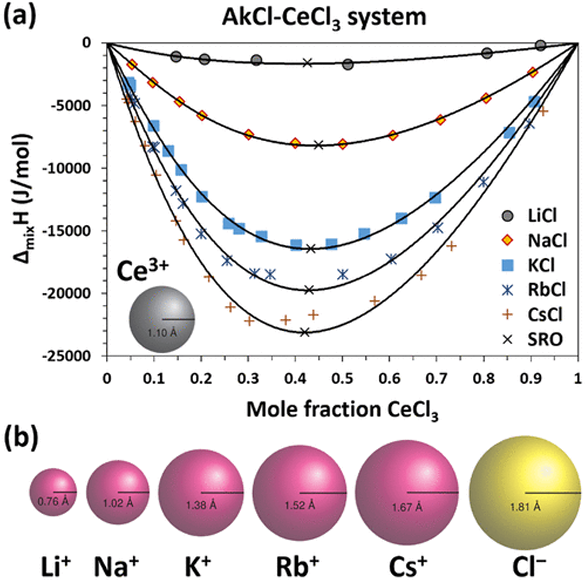
\includegraphics[width=0.4\textwidth]{chap2/image/12.1.png}
    \hfil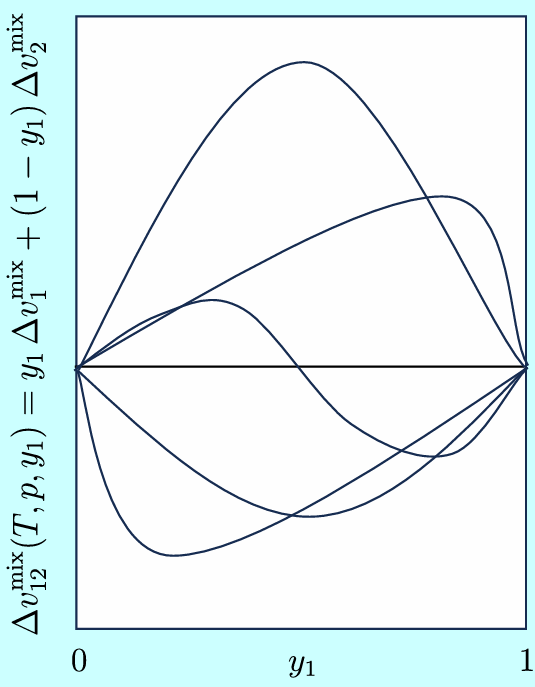
\includegraphics[width=0.33\textwidth]{chap2/image/12.2.png}
\end{center}
\begin{defn}
    \textbf{Partial properties} in terms of \textbf{partial pressures} and \textbf{pure-substance properties}
    \begin{zhu}
        partial pressure is not defined by a partial derivative 
        with respect to some amount at constant \(T\), \(p\), and \(\vec{n}\).
    \end{zhu}
    \begin{align*}
        s_i(T, p, \vec{y}) &= - \left( \frac{\partial \mu_i}{\partial T} \right)_{p, \vec{n}} 
        = - \left( \frac{\partial \mu_{ii}}{\partial T} \right)_{p, i} - \left( \frac{\partial \mu_{ii}}{\partial p_{ii}} \right)_T \left( \frac{\partial p_{ii}}{\partial T} \right)_{p, \vec{n}} \\
        &= s_{ii}(T, p_{ii}) - v_{ii}(T, p_{ii}) \, p_{ii,T}(T, p, \vec{y}) 
    \\
        v_i(T, p, \vec{y}) &= \left( \frac{\partial \mu_i}{\partial p} \right)_{T, \vec{n}} 
        = \left( \frac{\partial \mu_{ii}}{\partial p_{ii}} \right)_T \left( \frac{\partial p_{ii}}{\partial p} \right)_{T, \vec{y}} \\
        &= v_{ii}(T, p_{ii}) \, p_{ii,p}(T, p, \vec{y})
    \\
        h_i(T, p, \vec{y}) &= \mu_i(T, p, \vec{n}) + T \, s_i(T, p, \vec{y}) \\
        &= h_{ii}(T, p_{ii}) - T \, v_{ii}(T, p_{ii}) \, p_{ii,T}(T, p, \vec{y})
    \\
        u_i(T, p, \vec{y}) &= h_i(T, p, \vec{n}) - p \, v_i(T, p, \vec{y}) \\
        &= u_{ii}(T, p_{ii}) + v_{ii}(T, p_{ii}) \left[ p_{ii} - p_{ii,T}(T, p, \vec{y}) \, T - p_{ii,p}(T, p, \vec{y}) \, p \right]
    \end{align*}
\end{defn}








% 请你仔细转换为latex源码,使用align*环境

% 请你仔细转换为latex源码,使用gather*环境


%  ↑↑↑↑↑↑↑↑↑↑↑↑↑↑↑↑↑↑↑↑↑↑↑↑↑↑↑↑ 正文部分
\ifx\allfiles\undefined
\end{document}
\fi
